% 
% Annual Cognitive Science Conference
% Sample LaTeX Paper -- Proceedings Format
% 

% Original : Ashwin Ram (ashwin@cc.gatech.edu)       04/01/1994
% Modified : Johanna Moore (jmoore@cs.pitt.edu)      03/17/1995
% Modified : David Noelle (noelle@ucsd.edu)          03/15/1996
% Modified : Pat Langley (langley@cs.stanford.edu)   01/26/1997
% Latex2e corrections by Ramin Charles Nakisa        01/28/1997 
% Modified : Tina Eliassi-Rad (eliassi@cs.wisc.edu)  01/31/1998
% Modified : Trisha Yannuzzi (trisha@ircs.upenn.edu) 12/28/1999 (in process)
% Modified : Mary Ellen Foster (M.E.Foster@ed.ac.uk) 12/11/2000
% Modified : Ken Forbus                              01/23/2004
% Modified : Eli M. Silk (esilk@pitt.edu)            05/24/2005
% Modified : Niels Taatgen (taatgen@cmu.edu)         10/24/2006
% Modified : David Noelle (dnoelle@ucmerced.edu)     11/19/2014
% Modified : Roger Levy (rplevy@mit.edu)     12/31/2018



%% Change "letterpaper" in the following line to "a4paper" if you must.

\documentclass[10pt,letterpaper]{article}

\usepackage{cogsci}
\usepackage{xcolor}
\usepackage{graphicx}
\usepackage{amsmath}
\usepackage{amssymb}
\usepackage{subcaption}

\cogscifinalcopy % Uncomment this line for the final submission 


\usepackage{pslatex}
\usepackage{float} % Roger Levy added this and changed figure/table
                   % placement to [H] for conformity to Word template,
                   % though floating tables and figures to top is
                   % still generally recommended!

% Hyperlinked citations (blue links that jump to references)
% Note: hyperref must be loaded BEFORE apacite for compatibility
\usepackage[colorlinks=true,citecolor=blue,linkcolor=blue,urlcolor=blue]{hyperref}
\usepackage{apacite}

%\usepackage[none]{hyphenat} % Sometimes it can be useful to turn off
%hyphenation for purposes such as spell checking of the resulting
%PDF.  Uncomment this block to turn off hyphenation.


%\setlength\titlebox{4.5cm}
% You can expand the titlebox if you need extra space
% to show all the authors. Please do not make the titlebox
% smaller than 4.5cm (the original size).
%%If you do, we reserve the right to require you to change it back in
%%the camera-ready version, which could interfere with the timely
%%appearance of your paper in the Proceedings.

% Path to figures
\graphicspath{{media/result_plots/}{media/webapp_screenshots/}}


\title{Modeling Human Inference of Simple Dynamical Rules: \\ A Bayesian Program Induction Approach to Cellular Automata\thanks{Final Project Report (9.660)}}
 
\author{{\large \bf Blake Edwards (blakete@mit.edu)} \\
  Department of Aeronautics \& Astronautics, \\
  Massachusetts Institute of Technology, \\
  125 Massachusetts Ave, Cambridge, MA 02139, USA}


\begin{document}

\maketitle


\begin{abstract}
Humans can infer rich underlying structure from limited sequential data, often in ways that resemble approximate Bayesian inference over compositional hypothesis spaces. We investigate this capacity in a tightly controlled dynamical domain: one-dimensional binary cellular automata (1D CAs). Participants ($N=5$) completed a sequential prediction task in which they observed partial CA evolutions generated by unknown update rules and repeatedly predicted the next state from multiple-choice options with graded confidence ratings. In parallel, we implemented a resource-rational Bayesian program-induction model in Gen.jl that performs online inference over a grammar of Boolean CA rules using sequential Monte Carlo (SMC) with MCMC rejuvenation. We compared human predictions and confidence judgments to the model's posterior predictive distributions across time. Human behavior showed significant correlation with model predictions (Pearson $r = 0.39$), with both exhibiting increased confidence as evidence accumulated. Human accuracy (59\%) exceeded chance (25\%) but remained below the model (95\%), with the gap varying by rule complexity class. Together, our findings offer preliminary support for a Marr computational-level account of human online spatiotemporal inference as approximate Bayesian program induction over a compositional rule language, while highlighting the importance of resource-rational considerations. Code is available at \url{https://github.com/blakete/mit-9-660-final-project} and the experiment at \url{https://blakesnotes.io/9-660_CA_experiment/index.html}.

\textbf{Keywords:} 
cognition; probabilistic inference; Bayesian program induction; cellular automata; structure learning
\end{abstract}


%%%%%%%%%%%%%%%%%%%%%%%%%%%%%%%%%%%%%%%%%%%%%%%%%%%%%%%%%%%%%
\section{Introduction}
%%%%%%%%%%%%%%%%%%%%%%%%%%%%%%%%%%%%%%%%%%%%%%%%%%%%%%%%%%%%%

A central question in cognitive science concerns how humans learn structured rules from sparse sequential data. When we observe a physical system evolving over time (a bouncing ball, a spreading pattern, or even the behavior of another agent), we rapidly form hypotheses about the underlying dynamics and use these to predict future states. This capacity for \textit{structure learning} involves discovering the conditional dependence structure (the ``rule'') that best explains sequential observations, and it represents a core competency of human cognition \cite{tenenbaum2006theory}.

In this project, we investigate human rule inference in a tightly controlled dynamical domain: \textit{one-dimensional binary cellular automata} (1D CAs). Cellular automata provide an ideal model system for studying structure learning because they embody simple, deterministic dynamical laws that generate visually interpretable patterns ranging from trivial (uniform states) to complex (chaotic or computationally universal behavior). The 256 possible 1D CA rules can be represented as short Boolean programs over local neighborhoods, making them amenable to treatment as a Bayesian program induction problem \cite{wolfram1983statistical}.

\subsection{Theoretical Framework: Marr's Computational Level}

Following \citeA{marr1982vision}, we frame this project at the \textit{computational level} of analysis, asking what problem human cognition is solving and why. At this level, we hypothesize that humans perform approximate Bayesian inference over a structured hypothesis space of possible dynamical rules. The computational theory specifies:
\begin{enumerate}
    \item \textbf{Hypothesis space}: A compositional language of Boolean update rules (a ``language of thought'' for CA dynamics).
    \item \textbf{Prior}: A simplicity-biased distribution favoring shorter, more parsimonious rules.
    \item \textbf{Likelihood}: A probabilistic model of how rules generate observable state transitions.
    \item \textbf{Inference}: Sequential belief updating as new observations arrive.
\end{enumerate}

This framework builds on the foundational insight emphasized throughout computational cognitive science: that Bayesian inference over structured symbolic representations has strong explanatory power for human cognition \cite{griffiths2024bayesian}. Probabilistic models of cognition at Marr's computational level capture what problems the mind solves, leaving algorithmic and implementational details for subsequent investigation.

\subsection{Related Work}

Our approach connects to several influential research programs:

\subsubsection{Rational Rules and Language-of-Thought Models}
\citeA{Goodman2008} model concept learning as Bayesian inference over a grammar of logical rules, showing that syntactic complexity predicts learning difficulty. Our CA rule grammar is a direct analogue: a structured hypothesis space of Boolean expressions over local neighborhoods.

\subsubsection{Bayesian Program Induction}
\citeA{lake2015human} show that Bayesian inference over probabilistic programs can account for human-level one-shot concept learning. We apply the same computational-level idea to a dynamical domain where the ``programs'' are CA update rules and the data are their generated spacetime patterns.

\subsubsection{Online Spatiotemporal Pattern Learning}
Most relevantly, \citeA{mills2023spatiotemporal} show that in a 2D dot-trajectory prediction task, human sequential predictions are well-explained by a Bayesian program synthesis model using SMC with MCMC rejuvenation. Our 1D CA setting offers a simpler dynamical universe to examine whether human online inference mirrors the uncertainty dynamics of a Bayesian program learner.

\subsubsection{Resource-Rational Cognition}
\citeA{griffiths2024bayesian} emphasize that real human cognition operates under computational constraints. Resource-rational agents will systematically deviate from classical Bayesian rationality in ways consistent with observed human behavior. Our model incorporates resource-rational assumptions through limited particles, decision noise, and perceptual noise parameters.

\subsection{Research Questions}

We address two related questions:
\begin{enumerate}
    \item \textbf{Human-Model Alignment}: To what extent do human sequential predictions and confidence ratings align with a Bayesian program-induction model? Do humans update their uncertainty over CA rules in ways that resemble Bayesian posterior updating as more evidence accumulates?
    
    \item \textbf{Characterizing Discrepancies}: Where human behavior diverges from the model, can these discrepancies be attributed to differences in prior strength, decision noise, or approximate inference dynamics consistent with resource-rational cognition?
\end{enumerate}

\subsection{Contributions}
The main contributions of this work are:
\begin{itemize}
    \item We introduce a sequential CA prediction task with graded confidence ratings as a controlled paradigm for studying human inference of dynamical rules.
    \item We implement an online Bayesian program induction model over Boolean CA rules in Gen.jl using SMC with MCMC rejuvenation.
    \item We evaluate alignment between model posterior predictive uncertainty and human confidence dynamics across time and rule complexity classes.
\end{itemize}


%%%%%%%%%%%%%%%%%%%%%%%%%%%%%%%%%%%%%%%%%%%%%%%%%%%%%%%%%%%%%
\section{Methods}
%%%%%%%%%%%%%%%%%%%%%%%%%%%%%%%%%%%%%%%%%%%%%%%%%%%%%%%%%%%%%

\subsection{Domain: One-Dimensional Cellular Automata}

One-dimensional binary cellular automata evolve in discrete time steps over a binary array. At each time step $t$, the state of cell $i$ at time $t+1$ is determined by a local rule applied to a 3-cell neighborhood at time $t$:
\begin{equation}
    s_i^{t+1} = f(s_{i-1}^t, s_i^t, s_{i+1}^t)
\end{equation}
where $f: \{0,1\}^3 \rightarrow \{0,1\}$ is the update rule. We use periodic (wrap-around) boundary conditions, so $s_0^t = s_W^t$ and $s_{W+1}^t = s_1^t$. There are $2^{2^3} = 256$ possible rules, which are usually indexed and referred to by their ``Wolfram number'' \cite{wolfram1983statistical}.

These rules exhibit qualitatively different behaviors, classified by Wolfram into four classes:
\begin{itemize}
    \item \textbf{Class I}: Evolution to uniform state (e.g., Rule 32)
    \item \textbf{Class II}: Periodic structures (e.g., Rule 5, 108)
    \item \textbf{Class III}: Chaotic/aperiodic patterns (e.g., Rule 30, 60)
    \item \textbf{Class IV}: Complex, interacting structures (e.g., Rule 54, 110)
\end{itemize}

\begin{figure}[H]
\begin{center}
\begin{tabular}{cc}
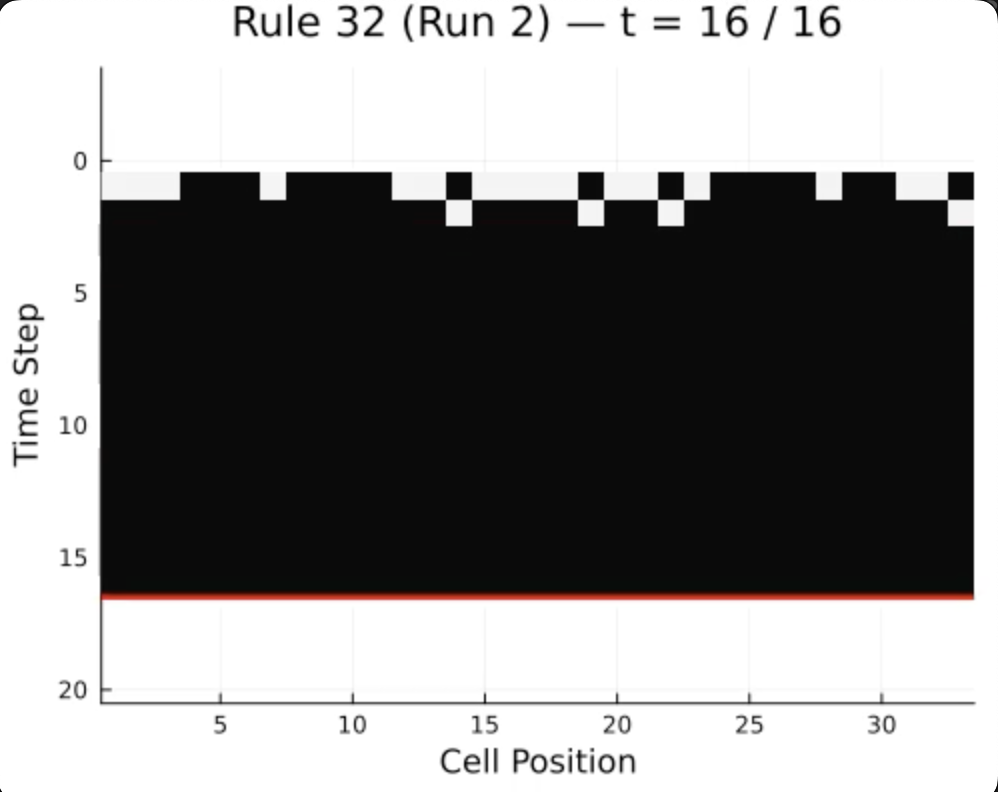
\includegraphics[width=0.42\columnwidth]{media/1D_CA_examples/class_I_rule_32.png} &
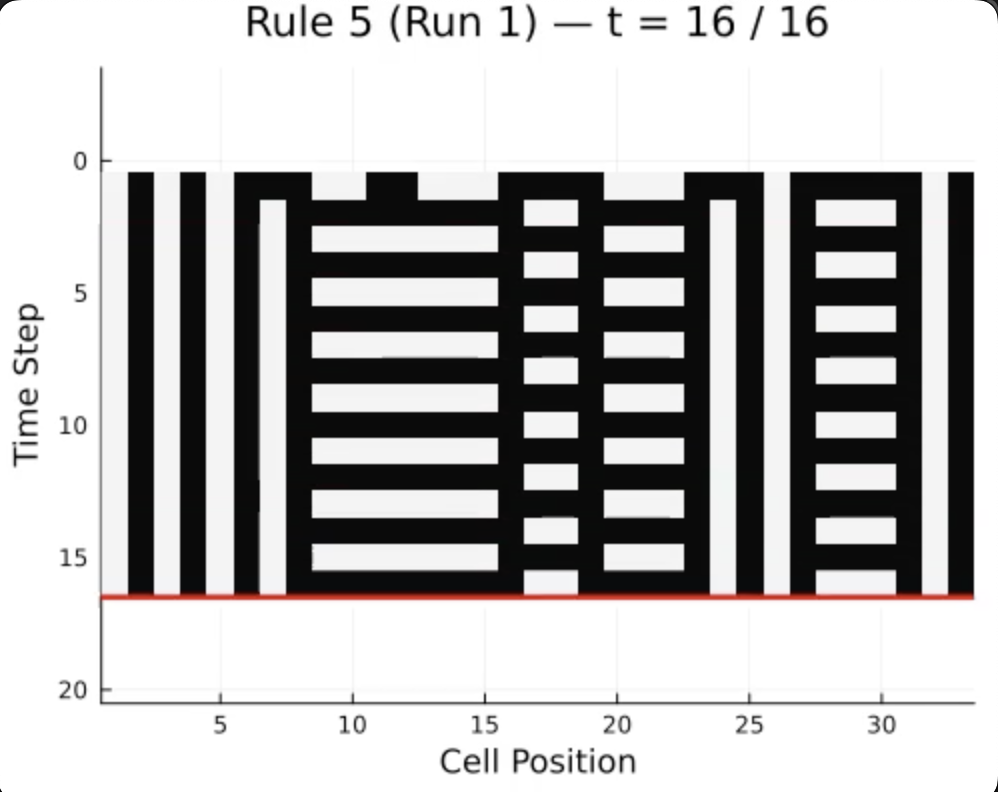
\includegraphics[width=0.42\columnwidth]{media/1D_CA_examples/class_II_rule_5.png} \\
\small (a) Class I: Rule 32 & \small (b) Class II: Rule 5 \\[0.5em]
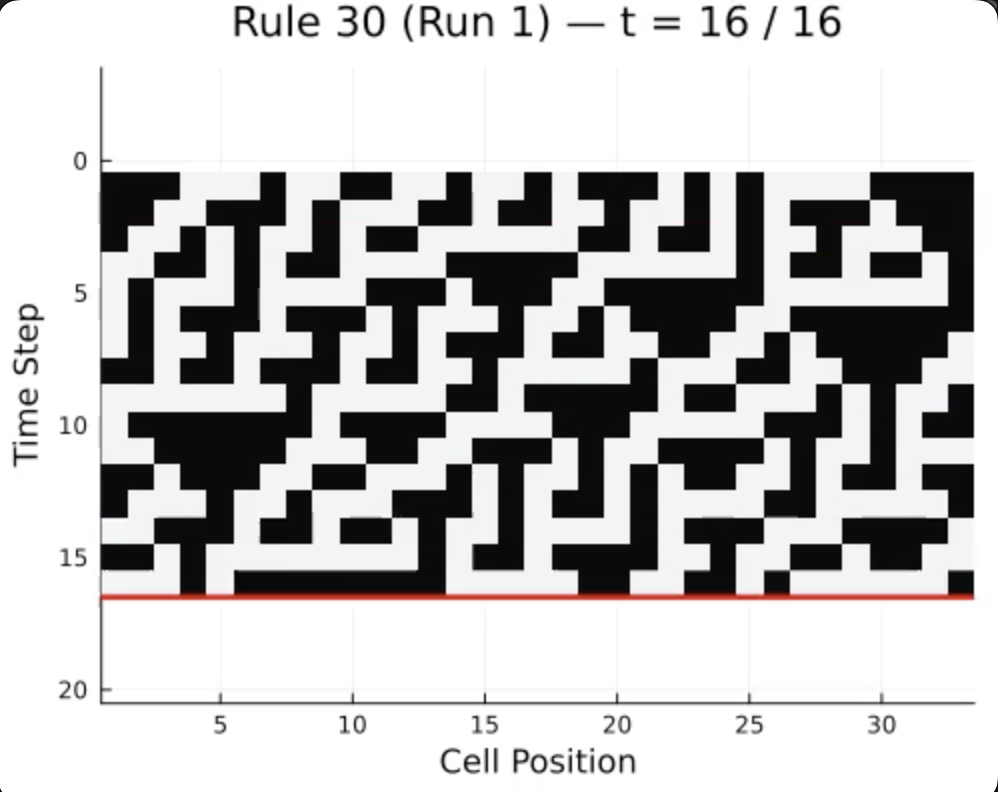
\includegraphics[width=0.42\columnwidth]{media/1D_CA_examples/class_III_rule_30.png} &
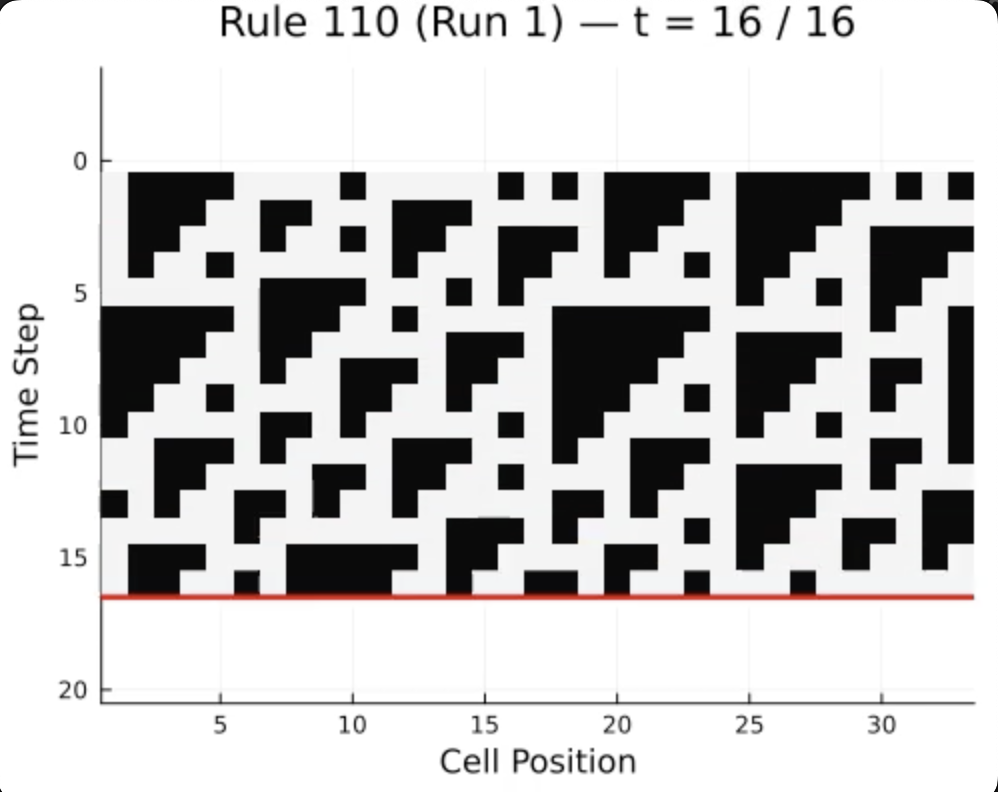
\includegraphics[width=0.42\columnwidth]{media/1D_CA_examples/class_IV_rule_110.png} \\
\small (c) Class III: Rule 30 & \small (d) Class IV: Rule 110
\end{tabular}
\end{center}
\caption{Examples of 1D cellular automata from each Wolfram class. Time evolves downward from an initial row. \textbf{(a)} Class I rules evolve to uniform states. \textbf{(b)} Class II rules produce periodic, repeating structures. \textbf{(c)} Class III rules generate chaotic, aperiodic patterns (Rule 30 is famously used for random number generation). \textbf{(d)} Class IV rules produce complex, interacting structures (Rule 110 is proven to be Turing complete).}
\label{fig:ca_classes}
\end{figure}

We selected 7 rules spanning all four classes for our experiment: Rules 5, 30, 32, 54, 60, 108, and 110 (see Appendix Figure~\ref{fig:all_rollouts}).

\subsection{Human Behavioral Experiment}

\subsubsection{Participants}
Five participants completed the experiment whose identities we will keep anonymous for the purposes of this report. All were friends or family members recruited through personal contacts.

\subsubsection{Stimuli}
For each of the 7 CA rules, we generated spacetime diagrams showing $t$ rows of CA evolution (width = 17 cells). Initial rows were selected manually from a pre-generated ``zoo'' of CA patterns to ensure visually informative evolutions.

\subsubsection{Task Structure and Interface}
The experiment was implemented as a mobile-friendly browser-based web application (Figure~\ref{fig:webapp}). Participants first watched a 30-second tutorial video explaining the task, then completed 42 trials ($7 \text{ rules} \times 6 \text{ time steps}$).

\begin{figure}[H]
\begin{center}
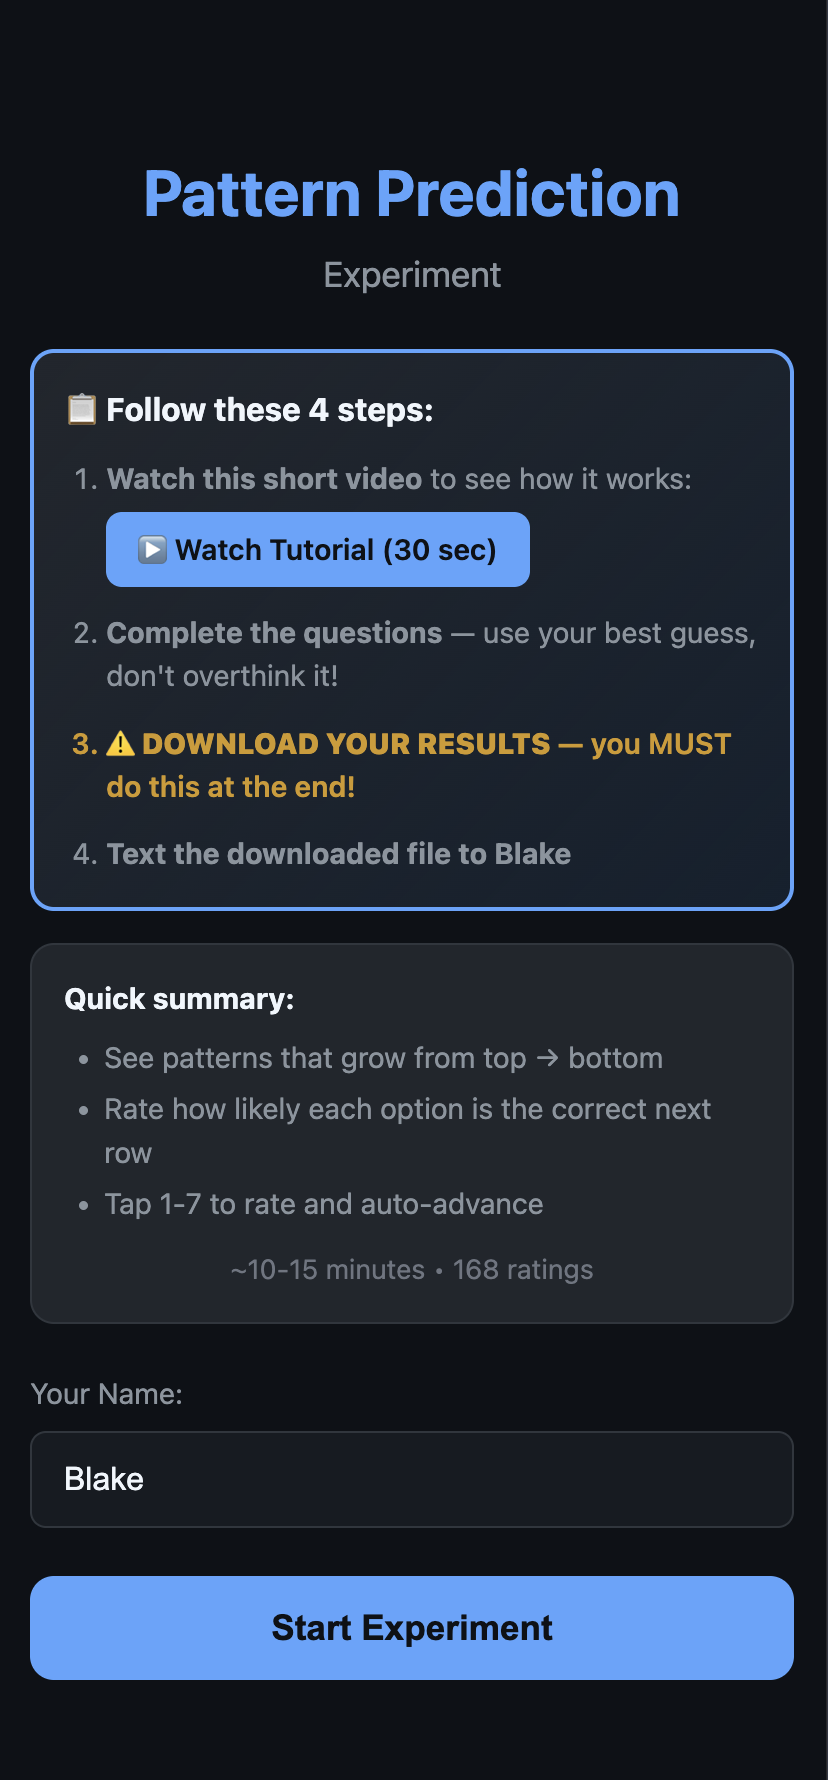
\includegraphics[width=0.48\columnwidth]{media/webapp_screenshots/start_page.png}
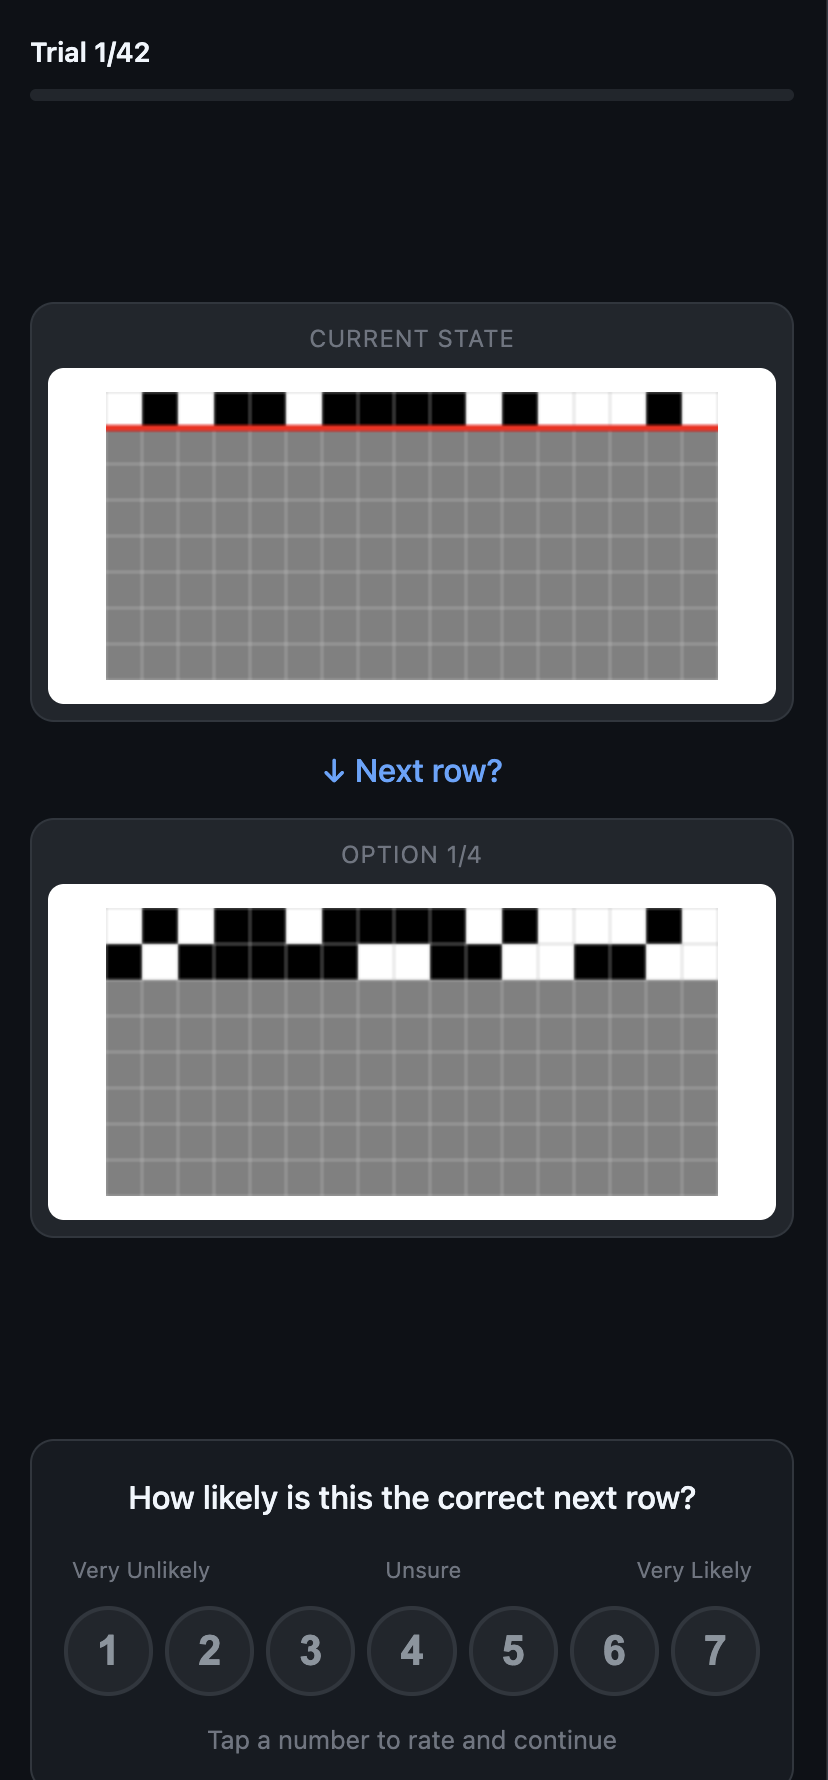
\includegraphics[width=0.48\columnwidth]{media/webapp_screenshots/q1_t1.png}
\end{center}
\caption{Web application interface. \textbf{Left}: Start page with instructions and tutorial video link. Participants were told to ``see patterns that grow from top $\rightarrow$ bottom'' and ``rate how likely each option is the correct next row.'' \textbf{Right}: Trial interface showing the current CA state (top panel with red prediction boundary) and one answer option (bottom panel). Participants rated each of four options on a 1--7 scale.}
\label{fig:webapp}
\end{figure}

Each trial presented:
\begin{enumerate}
    \item A \textbf{current state image} showing $t$ rows of CA evolution (where $t \in \{1, 2, 3, 4, 5, 6\}$), with the next row position indicated by a red prediction boundary and gray cells representing the unknown future.
    \item Four \textbf{answer options} shown sequentially, each displaying what the CA would look like with a different candidate next row.
\end{enumerate}

The four options consisted of:
\begin{itemize}
    \item The \textbf{correct} next row (from the true generating rule)
    \item A \textbf{numerically adjacent} rule (rule number $\pm 1$)
    \item A rule from the \textbf{same Wolfram class}
    \item A \textbf{randomly selected} rule from 0--255
\end{itemize}

Participants rated each option on a 1--7 Likert scale indicating their confidence that it was the correct continuation (1 = Very Unlikely, 4 = Unsure, 7 = Very Likely). Tapping a number automatically advanced to the next option. The experiment took approximately 10--15 minutes to complete, with 168 total ratings per participant ($42 \text{ trials} \times 4 \text{ options}$).

\begin{figure}[H]
\begin{center}
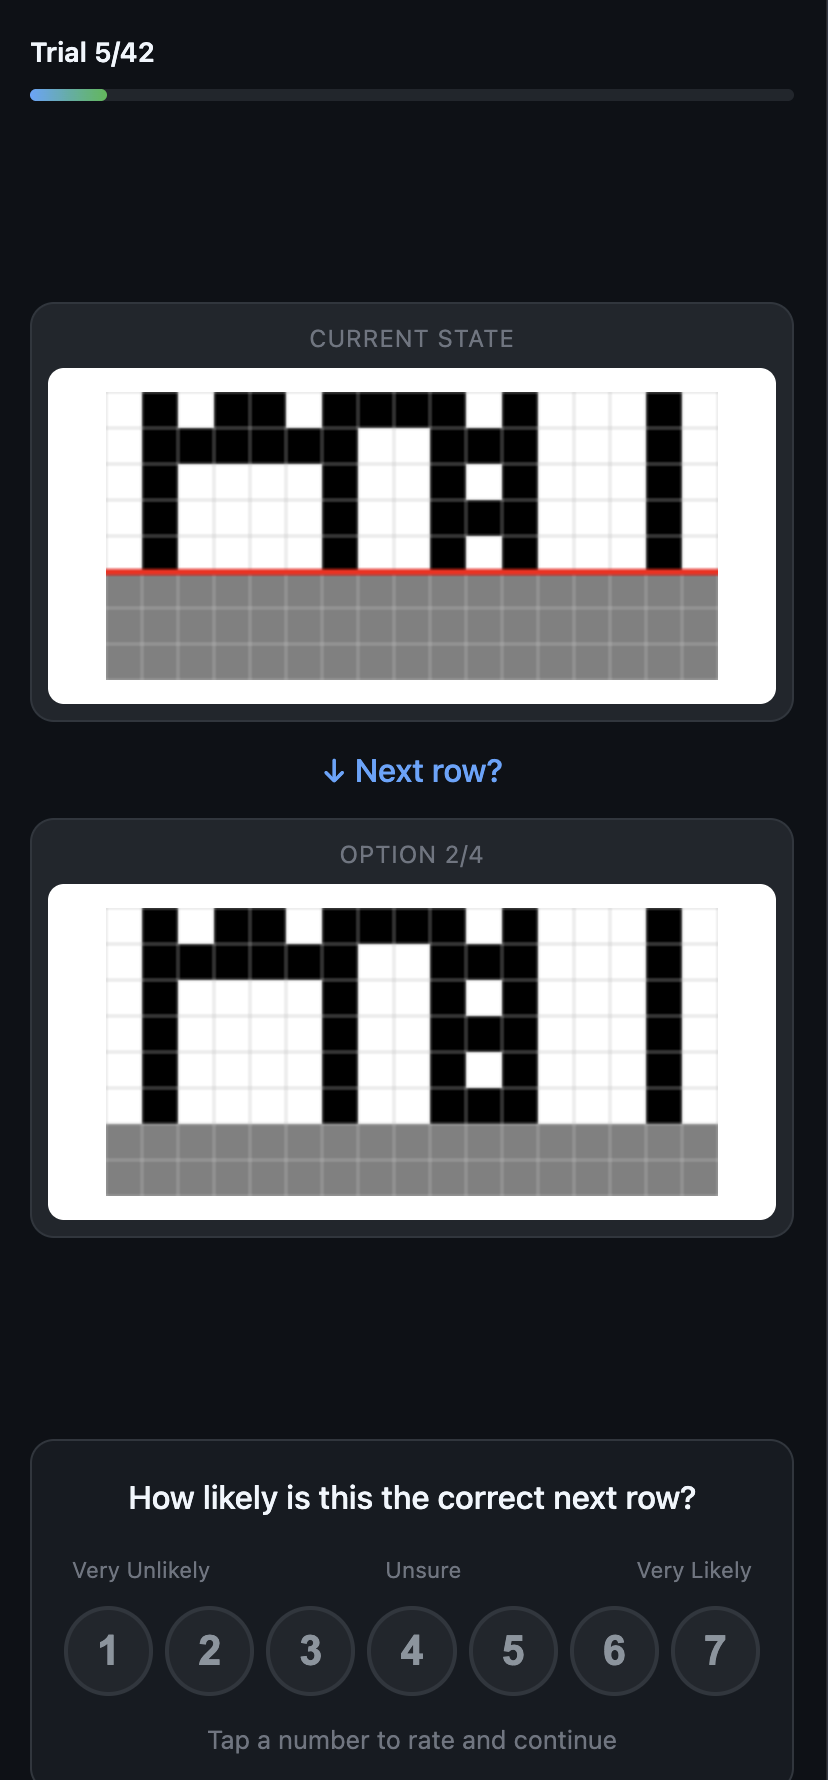
\includegraphics[width=0.48\columnwidth]{media/webapp_screenshots/q1_t6.png}
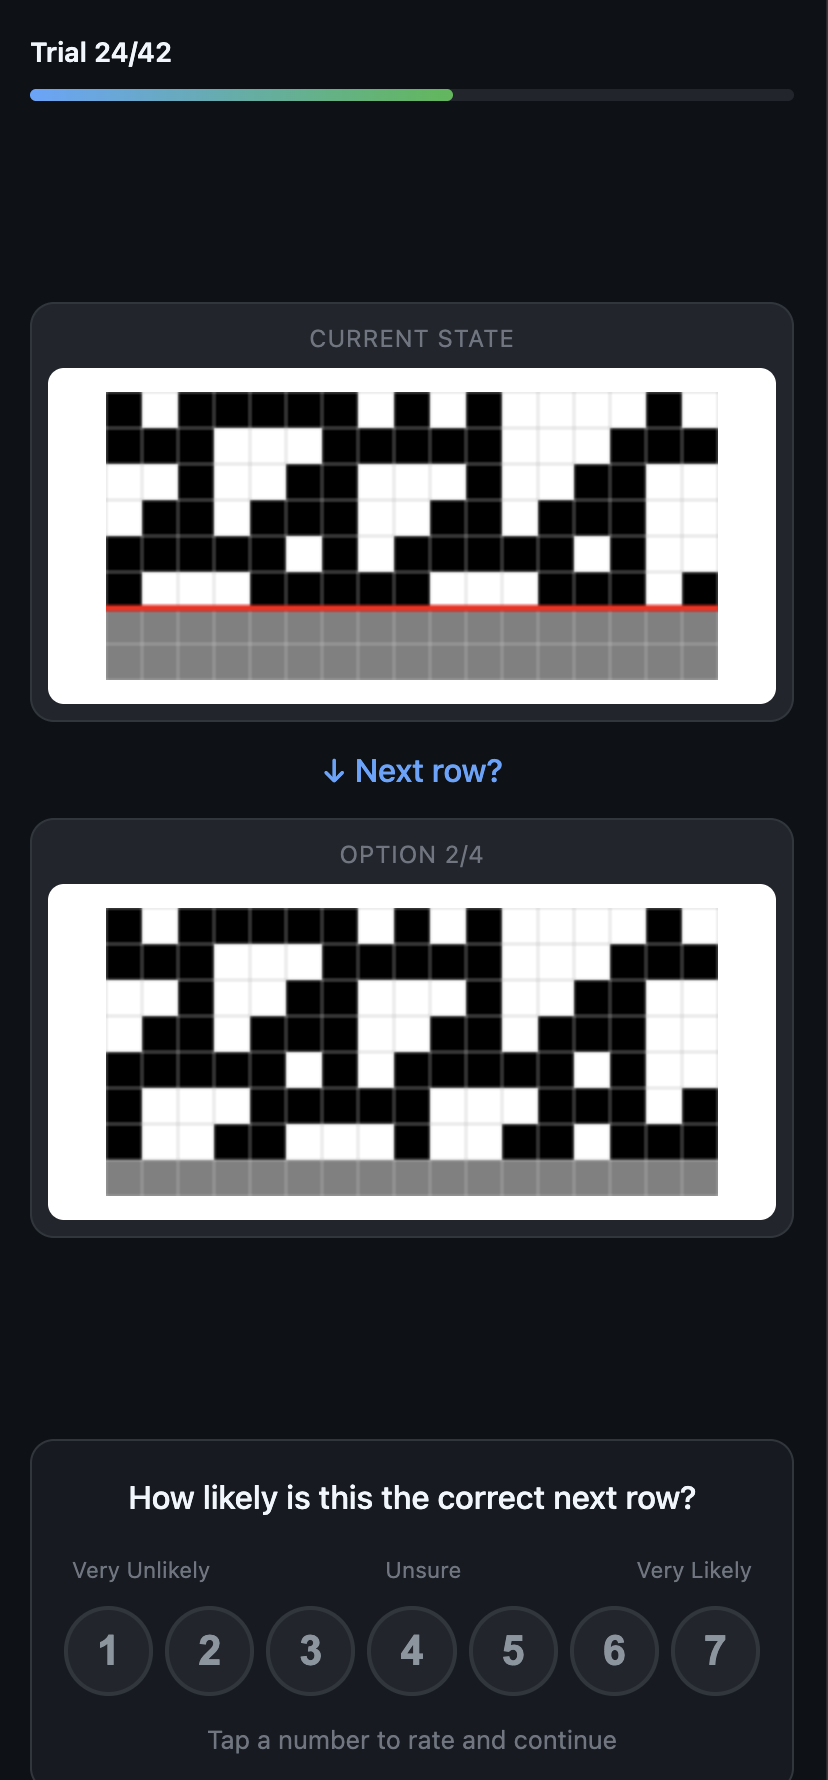
\includegraphics[width=0.48\columnwidth]{media/webapp_screenshots/q4_t6.png}
\end{center}
\caption{Example trials at $t=6$ showing more evolved CA patterns. \textbf{Left}: A periodic rule showing regular structure. \textbf{Right}: A chaotic rule showing complex, irregular patterns. The prediction task becomes easier with more evidence (rows), but chaotic rules remain challenging.}
\label{fig:trials_t6}
\end{figure}

\subsubsection{Procedure}
Participants accessed the experiment via a URL on their personal devices. They were instructed that they would see patterns evolving according to hidden rules and should predict the most likely next row. No feedback was provided during the experiment. At the end, participants downloaded their results as a JSON file and submitted it to the experimenter.

\subsection{Bayesian Program-Induction Model}

\subsubsection{Rule Representation: A Grammar of Boolean Programs}
We represent CA rules as abstract syntax trees (ASTs) generated from a probabilistic context-free grammar over Boolean expressions:

\begin{itemize}
    \item \textbf{Atoms} (leaves): \texttt{left}, \texttt{center}, \texttt{right} (neighborhood inputs), \texttt{one}, \texttt{zero} (constants)
    \item \textbf{Unary operator}: \texttt{not}
    \item \textbf{Binary operators}: \texttt{and}, \texttt{or}, \texttt{xor}
\end{itemize}

For example, Rule 60 (XOR of left and center) can be expressed as \texttt{xor(left, center)}.

\subsubsection{Grammar Prior}
The grammar uses a geometric prior on tree size controlled by parameter $p_{\text{leaf}} = 0.5$:
\begin{itemize}
    \item With probability $p_{\text{leaf}}$, generate an atom uniformly from \{\texttt{left}, \texttt{center}, \texttt{right}, \texttt{zero}, \texttt{one}\}
    \item With probability $(1 - p_{\text{leaf}}) \cdot 0.2$, generate a \texttt{not} node and recurse
    \item With probability $(1 - p_{\text{leaf}}) \cdot 0.8$, generate a binary operator uniformly from \{\texttt{and}, \texttt{or}, \texttt{xor}\} and recurse on both children
\end{itemize}

This grammar can express all 256 Wolfram rules, though with redundancy: multiple syntactically distinct trees may be extensionally equivalent (e.g., \texttt{and(left, center)} and \texttt{and(center, left)}). We do not explicitly handle this redundancy, allowing the posterior to distribute mass across equivalent representations. This prior favors simpler (shorter) rules, implementing a ``simplicity bias'' analogous to that used in rational rules models \cite{Goodman2008}.

\subsubsection{Likelihood Function}
Given a rule tree $r$ and observed transition from row $\mathbf{s}^t$ to $\mathbf{s}^{t+1}$, we compute the likelihood with noise parameter $\varepsilon$:
\begin{equation}
    P(\mathbf{s}^{t+1} | \mathbf{s}^t, r) = \prod_{i=1}^{W} 
    \begin{cases}
        1 - \varepsilon & \text{if } s_i^{t+1} = f_r(s_{i-1}^t, s_i^t, s_{i+1}^t) \\
        \varepsilon & \text{otherwise}
    \end{cases}
\end{equation}
where $W = 17$ is the CA width.

\subsubsection{Sequential Monte Carlo Inference}
We implemented online Bayesian inference using Sequential Monte Carlo (SMC) with MCMC rejuvenation in Gen.jl \cite{cusumano2019gen}, following \citeA{saad2019bayesian} and \citeA{saad2023smc}. Algorithm~\ref{alg:smc} provides pseudo-code for the inference procedure.

\begin{figure}[H]
\small
\begin{tabular}{p{0.95\columnwidth}}
\hline
\textbf{Algorithm 1}: SMC for CA Rule Inference \\
\hline
\textbf{Input}: Observations $\mathbf{s}^1, \ldots, \mathbf{s}^{T+1}$; particles $N$; noise $\varepsilon$ \\
\textbf{Output}: Posterior samples $\{r_i\}_{i=1}^N$ over rule trees \\[0.3em]
1. \textbf{Initialize}: Sample $r_i \sim \text{Grammar}(p_{\text{leaf}})$ for $i = 1, \ldots, N$ \\
\quad Set weights $w_i \leftarrow 0$ \\[0.3em]
2. \textbf{For} $t = 1$ to $T$: \\
\quad 2a. \textbf{Weight Update}: \\
\quad\quad $w_i \leftarrow w_i + \log P(\mathbf{s}^{t+1} | \mathbf{s}^t, r_i; \varepsilon)$ \\[0.2em]
\quad 2b. \textbf{Resample} if ESS $< N/2$: \\
\quad\quad Draw $\{r_i'\}$ from $\{r_i\}$ with prob. $\propto \exp(w_i)$ \\
\quad\quad Reset $w_i \leftarrow 0$ \\[0.2em]
\quad 2c. \textbf{Rejuvenate} (for each particle, $K$ steps): \\
\quad\quad Propose $r' \sim q(r' | r_i)$ via structure move \\
\quad\quad Accept with MH ratio including likelihood \\[0.3em]
3. \textbf{Predict}: For candidate row $\mathbf{c}$, return \\
\quad $P(\mathbf{c}) = \frac{1}{N} \sum_i \mathbf{1}[f_{r_i}(\mathbf{s}^t) = \mathbf{c}]$ \\
\hline
\end{tabular}
\label{alg:smc}
\end{figure}

The rejuvenation step (2c) applies $K=3$ Metropolis-Hastings moves per particle to maintain diversity. We use five structure-modifying proposals:
\begin{itemize}
    \item \textbf{Grow}: Replace a random atom with a binary subtree
    \item \textbf{Prune}: Replace a random subtree with an atom
    \item \textbf{Swap-Op}: Change the operator at a binary node
    \item \textbf{Swap-Atom}: Change the type of a leaf node
    \item \textbf{Toggle-Not}: Add or remove a negation wrapper
\end{itemize}
Each rejuvenation step selects one of the five proposal types uniformly at random. Proposals are accepted or rejected using the Metropolis-Hastings criterion with the full posterior (likelihood $\times$ prior ratio), ensuring that rejuvenation moves particles toward higher-probability rule trees while maintaining detailed balance. With $N = 20$ particles and $K = 3$ moves per particle, this yields 60 total MCMC steps per time step. Empirically, acceptance rates ranged from approximately 15--40\% depending on the proposal type and posterior concentration.

\subsubsection{Resource-Rational Parameterization}
To model bounded human cognition, we used deliberately constrained inference parameters:
\begin{itemize}
    \item \textbf{Limited particles} ($N = 20$): Reflects working memory constraints, since humans cannot maintain hundreds of hypotheses simultaneously
    \item \textbf{High perceptual noise} ($\varepsilon = 0.20$): Models attention and perception errors when processing the CA grid
    \item \textbf{Few rejuvenation steps} ($K = 3$): Limits hypothesis refinement per observation
    \item \textbf{Decision noise}: Power-law temperature $\tau = 3.0$ applied to choice probabilities via $P_{\text{choice}}(i) \propto P_{\text{model}}(i)^{1/\tau}$, modeling stochastic response selection
\end{itemize}

\subsection{Model-Human Comparison}

We compared human and model responses using several metrics:
\begin{itemize}
    \item \textbf{Accuracy}: Whether the highest-rated option (human) or highest-probability option (model) was correct. We computed two accuracy measures: \textit{rule-based accuracy}, which counts a response as correct only if it matches the true Wolfram rule number, and \textit{manifest-based accuracy}, which counts a response as correct if the chosen option produces the same \textit{manifest} next row, meaning the same observable pattern of black and white cells, as the true rule would produce for the given initial condition. This distinction matters because different Wolfram rules can be \textit{extensionally equivalent} for a particular initial state, producing identical next rows despite having different underlying Boolean expressions. Manifest-based accuracy is arguably the fairer measure, as it credits participants for selecting visually indistinguishable options.
    \item \textbf{Correlation}: Pearson and Spearman correlations between human ratings and model probabilities across all option$\times$trial combinations ($N = 840$ datapoints).
    \item \textbf{KL Divergence}: $D_{KL}(\text{Human} \| \text{Model})$ measuring distributional similarity.
\end{itemize}

Human ratings were converted to probabilities using softmax normalization (temperature = 1.5) centered at the scale midpoint.


%%%%%%%%%%%%%%%%%%%%%%%%%%%%%%%%%%%%%%%%%%%%%%%%%%%%%%%%%%%%%
\section{Results}
%%%%%%%%%%%%%%%%%%%%%%%%%%%%%%%%%%%%%%%%%%%%%%%%%%%%%%%%%%%%%

\subsection{Overall Performance}

Aggregating across all 5 participants and 42 trials each (210 total trial responses, 840 individual ratings):

\begin{itemize}
    \item \textbf{Human accuracy (rule-based)}: 47.1\% (chance = 25\%)
    \item \textbf{Human accuracy (manifest-based)}: 58.6\%
    \item \textbf{Model accuracy}: 95.2\%
    \item \textbf{Human-model correlation}: Pearson $r = 0.39$, Spearman $\rho = 0.33$ (computed over all option$\times$trial pairs; inferential statistics should be interpreted cautiously due to repeated-measures structure with ratings nested within participants and trials)
    \item \textbf{KL divergence}: Mean $D_{KL}(\text{Human} \| \text{Model}) = 1.47$ (SD $= 1.63$), indicating moderate distributional divergence between human probability judgments and model posteriors.
\end{itemize}

The manifest-based accuracy accounts for the fact that different Wolfram rules can produce identical next rows for a given initial condition, crediting humans when they choose any ``correct-looking'' option. The correlation shows that human predictions track model predictions at a coarse level: options that the Bayesian model considers likely tend to receive higher human ratings.

\subsection{Temporal Dynamics: Evidence Accumulation}

A key prediction of Bayesian updating is that confidence should increase as evidence accumulates. We examined accuracy and confidence across time steps $t \in \{1, ..., 6\}$.

\begin{figure}[H]
\begin{center}
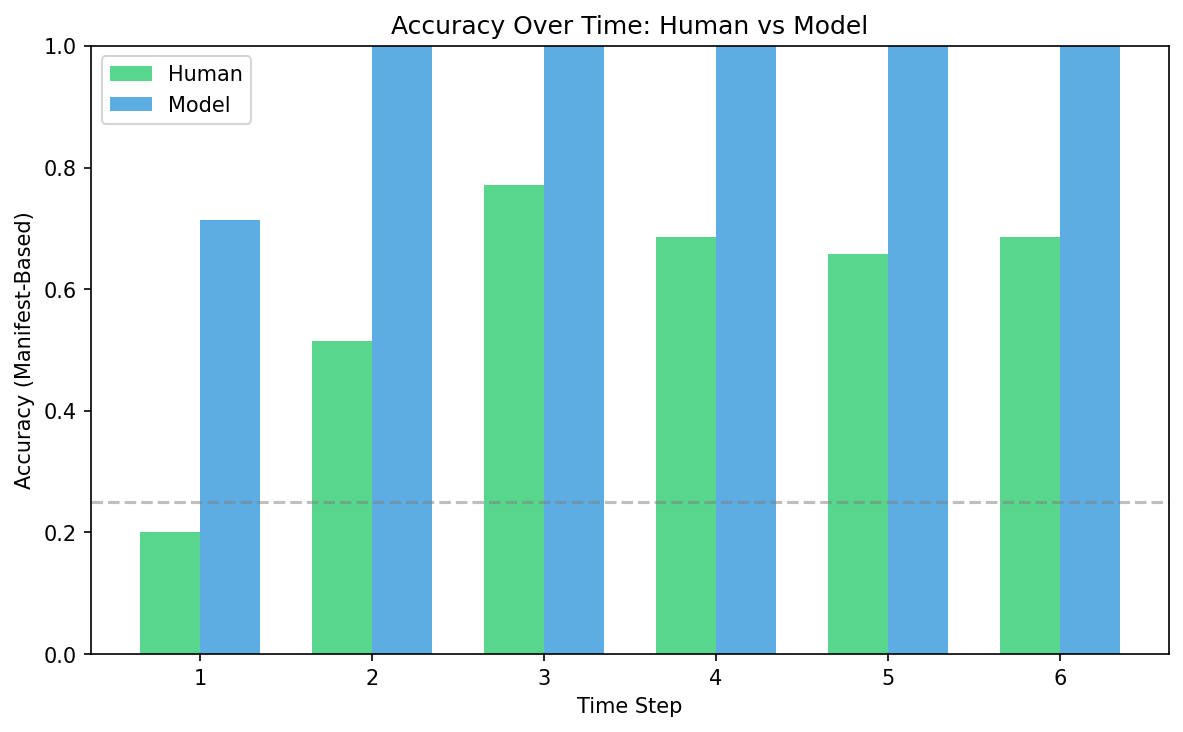
\includegraphics[width=0.95\columnwidth]{media/results/accuracy_by_time.png}
\end{center}
\caption{Accuracy over time steps. Both human (green) and model (blue) accuracy exceed chance (25\%, dashed line). Human accuracy increases dramatically from $t=1$ (20\%) to $t=3$ (77\%), then plateaus around 65--70\%. The model achieves near-perfect accuracy after $t=1$.}
\label{fig:accuracy_time}
\end{figure}

\begin{figure}[H]
\begin{center}
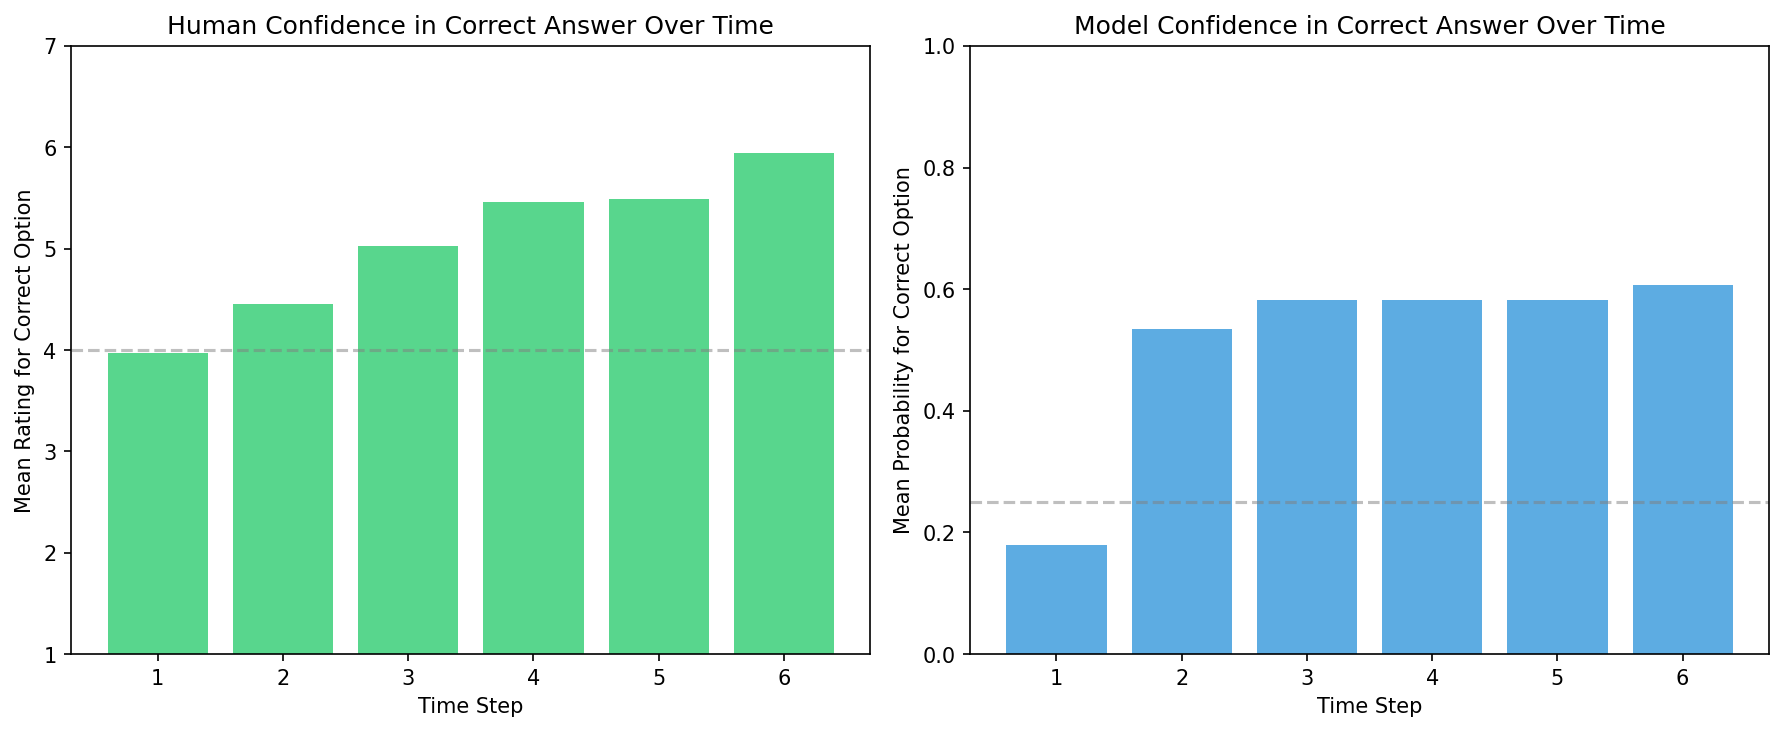
\includegraphics[width=0.95\columnwidth]{media/results/correct_option_confidence.png}
\end{center}
\caption{Confidence in the correct option over time. \textbf{Left}: Mean human rating for the correct answer increases steadily from $\sim$4 (unsure) at $t=1$ to $\sim$6 (likely) at $t=6$. \textbf{Right}: Model probability assigned to the correct option also increases, but more rapidly, plateauing after $t=2$. Both exhibit evidence accumulation consistent with Bayesian updating.}
\label{fig:confidence}
\end{figure}

The temporal dynamics reveal important patterns:
\begin{itemize}
    \item At $t=1$, humans perform near chance (20\%) with neutral confidence (rating $\approx$ 4), consistent with high uncertainty when only one row is observed.
    \item Human accuracy and confidence increase monotonically with time, consistent with sequential evidence accumulation.
    \item The model reaches high confidence faster than humans, suggesting either more efficient inference or less conservative probability assignments.
\end{itemize}

\begin{figure}[H]
\begin{center}
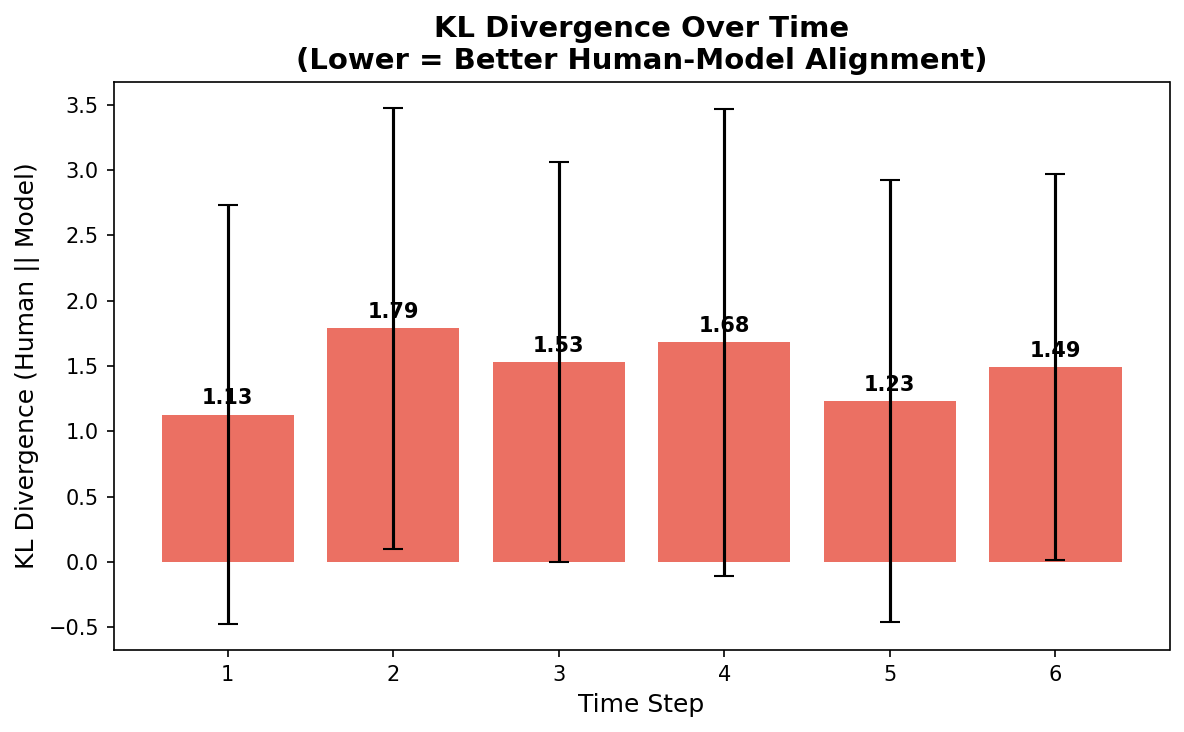
\includegraphics[width=0.75\columnwidth]{media/results/kl_by_time.png}
\end{center}
\caption{KL divergence between human and model probability distributions over time steps. Lower values indicate better alignment. KL divergence remains relatively stable across time steps (ranging from 1.13 to 1.79), suggesting that while both humans and model converge toward the correct answer, they do so with persistently different distributional shapes.}
\label{fig:kl_time}
\end{figure}

The KL divergence between human and model distributions does not decrease monotonically over time (Figure~\ref{fig:kl_time}). Even as both humans and the model become more accurate, they maintain different uncertainty profiles: the model tends toward sharper, more confident predictions while humans retain broader distributions.

\subsection{Performance by Rule Class}

CA rules from different Wolfram classes exhibit different dynamics. We examined whether human and model performance varied across classes.

\begin{figure}[H]
\begin{center}
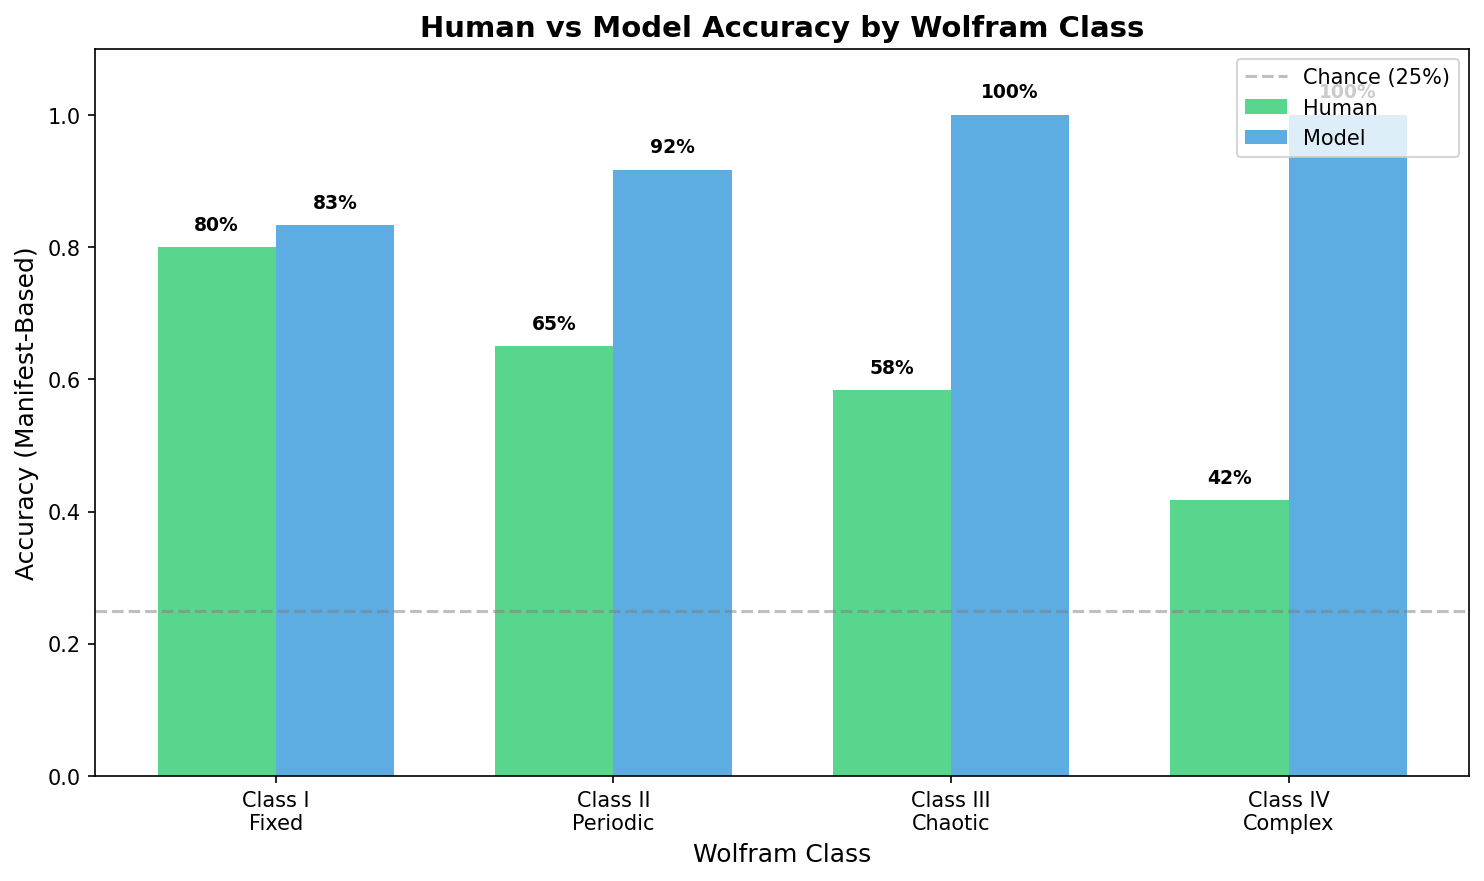
\includegraphics[width=0.95\columnwidth]{media/results/human_vs_model_by_class.png}
\end{center}
\caption{Accuracy by Wolfram class (manifest-based). Both human and model performance varies by class: Class I (Fixed) rules are easiest (80\% human, 83\% model), while Class IV (Complex) rules are hardest (42\% human, though model achieves 100\%). The human-model gap increases with rule complexity.}
\label{fig:accuracy_class}
\end{figure}

\begin{figure}[H]
\begin{center}
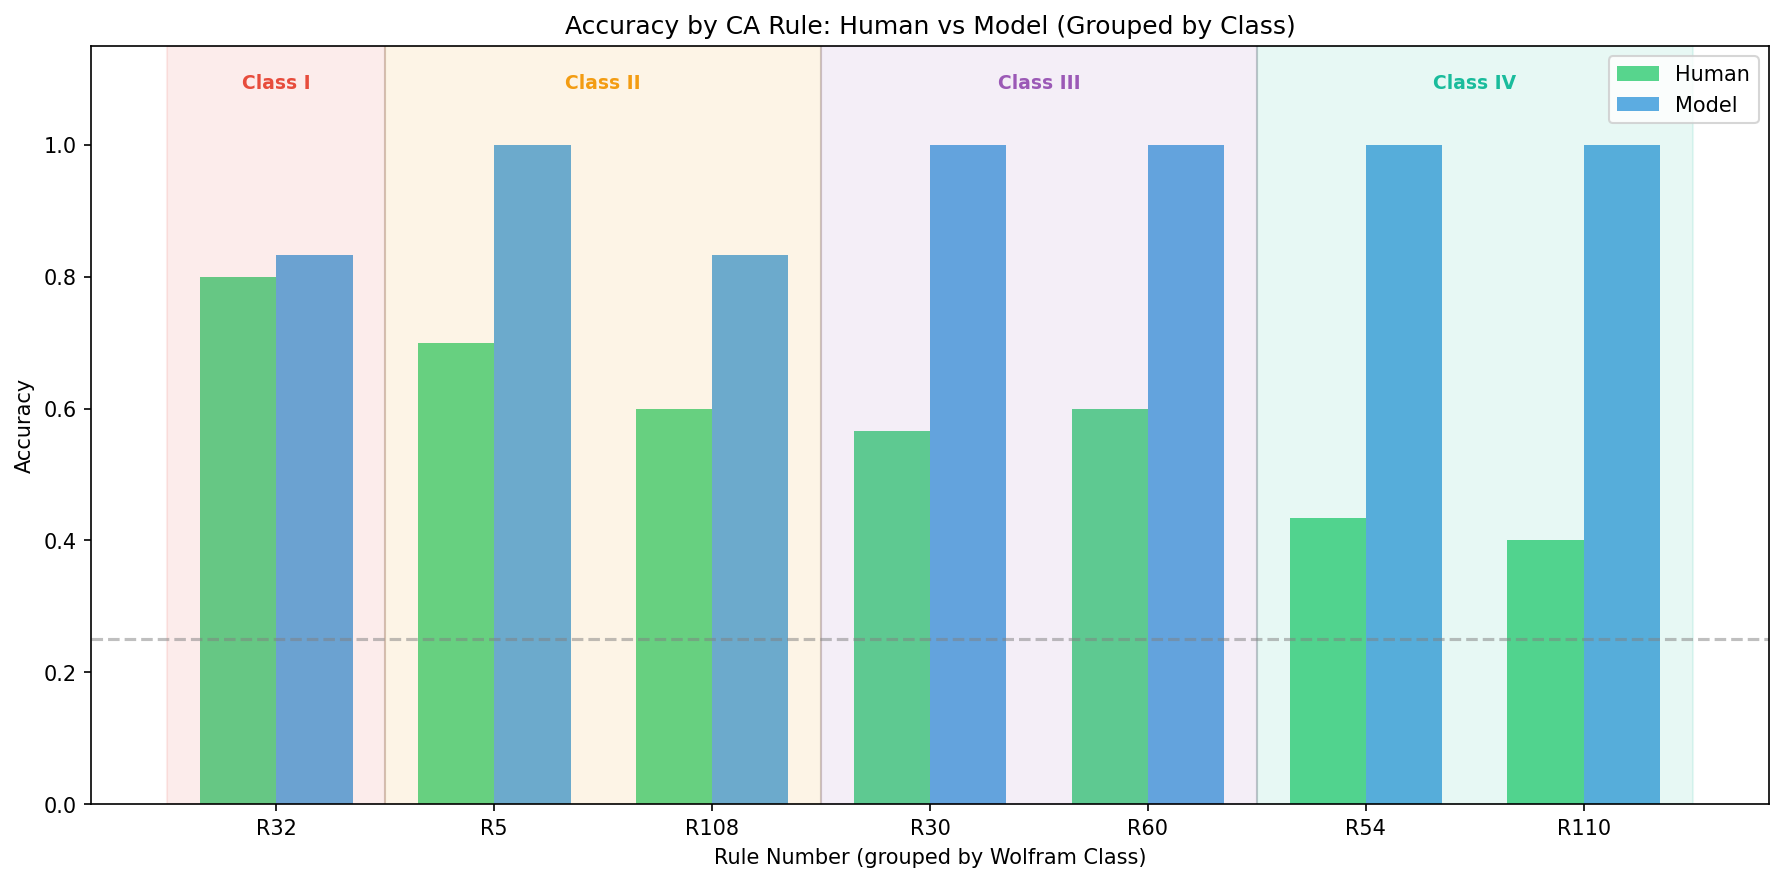
\includegraphics[width=0.95\columnwidth]{media/results/accuracy_by_rule.png}
\end{center}
\caption{Accuracy by individual CA rule, grouped by Wolfram class. Background colors indicate class (red = Class I, yellow = Class II, purple = Class III, teal = Class IV). Human accuracy varies across rules even within the same class.}
\label{fig:accuracy_rule}
\end{figure}

Notable patterns include:
\begin{itemize}
    \item \textbf{Class I (Fixed)}: Both human (80\%) and model (83\%) perform well. Rule 32 produces predictable patterns that are easy to extrapolate.
    \item \textbf{Class II (Periodic)}: Humans achieve 65\% accuracy, with Rule 5 (70\%) easier than Rule 108 (60\%). The model achieves 92\%.
    \item \textbf{Class III (Chaotic)}: Despite the chaotic dynamics, humans achieve 58\% accuracy. The model achieves 100\%, suggesting the chaotic patterns are actually highly constraining (few rules produce the same chaotic output).
    \item \textbf{Class IV (Complex)}: The largest human-model gap appears here: humans achieve only 42\% while the model achieves 100\%. Rules 54 and 110 produce complex patterns that are difficult for humans to predict but distinguishable for the model.
\end{itemize}

\begin{figure}[H]
\begin{center}
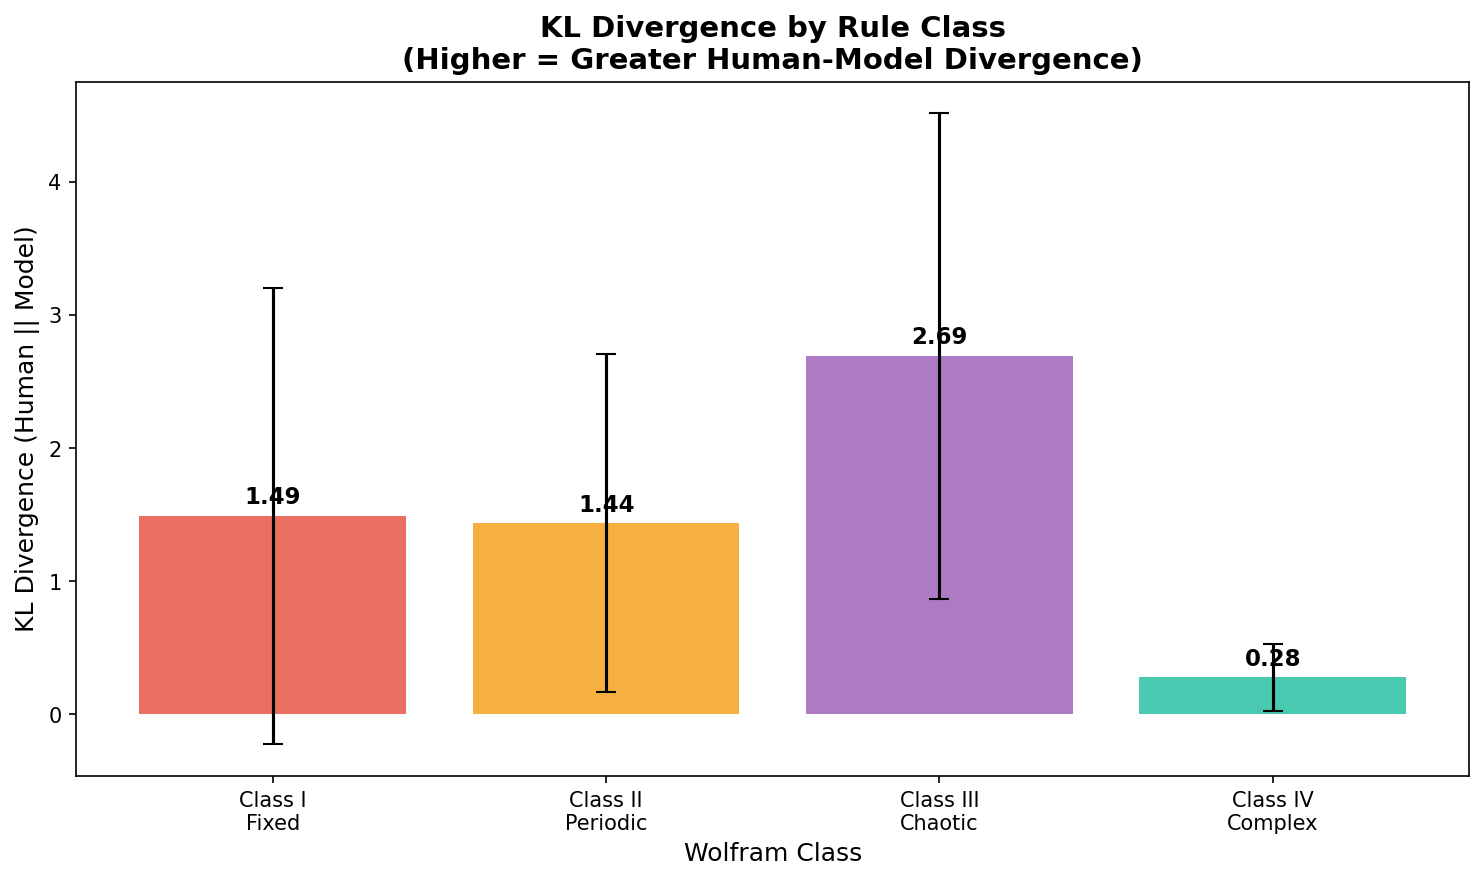
\includegraphics[width=0.75\columnwidth]{media/results/kl_by_class.png}
\end{center}
\caption{KL divergence between human and model distributions by Wolfram class. Higher KL indicates greater distributional divergence. Class III (Chaotic) shows the highest KL divergence (2.69), while Class IV (Complex) shows the lowest (0.28).}
\label{fig:kl_class}
\end{figure}

The KL divergence analysis (Figure~\ref{fig:kl_class}) reveals a surprising pattern: Class III (Chaotic) rules show the \textit{highest} distributional divergence between human and model ($D_{KL} = 2.69$), while Class IV (Complex) rules show the \textit{lowest} ($D_{KL} = 0.28$). For chaotic rules, humans and the model arrive at correct answers through different probability assignments. The model achieves 100\% accuracy with sharp posteriors, while humans spread probability mass more diffusely. For complex rules, despite the large accuracy gap, humans who do engage with the task appear to assign probabilities in patterns more similar to the model's posterior.


%%%%%%%%%%%%%%%%%%%%%%%%%%%%%%%%%%%%%%%%%%%%%%%%%%%%%%%%%%%%%
\section{Discussion}
%%%%%%%%%%%%%%%%%%%%%%%%%%%%%%%%%%%%%%%%%%%%%%%%%%%%%%%%%%%%%

\subsection{Summary of Findings}

This project investigated whether human inference of dynamical rules from sequential CA observations could be characterized as approximate Bayesian program induction. Our main findings were:

\begin{enumerate}
    \item \textbf{Significant human-model correlation}: Human ratings showed significant positive correlation ($r = 0.39$) with Bayesian model probabilities, suggesting that human inferences track the posterior predictive distribution at a coarse level.
    
    \item \textbf{Evidence accumulation}: Both humans and the model showed increasing confidence in correct answers over time, consistent with sequential Bayesian updating (Figure~\ref{fig:confidence}).
    
    \item \textbf{Accuracy gap varies by complexity}: The model outperformed humans, but the gap varied by rule class, smallest for simple fixed-point rules (3\% gap) and largest for complex Class IV rules (58\% gap).
    
    \item \textbf{Above-chance human performance}: Humans exceeded chance (25\%) on all rule classes, showing genuine structure learning.
\end{enumerate}

\subsection{What Worked}

% [Topic: Experimental paradigm]
The browser-based mobile interface proved effective, enabling rapid data collection with minimal friction. The sequential presentation of options with 1--7 ratings captured graded confidence judgments rather than just forced choices.

% [Topic: Model-human alignment]
The correlation between human ratings and model probabilities supports the basic hypothesis that humans engage in structure learning over CA rules. The temporal dynamics, particularly the monotonic increase in confidence from $t=1$ to $t=6$, suggest that humans update beliefs sequentially in a manner consistent with Bayesian inference.

% [Topic: Rule class effects]
Performance varied across Wolfram classes, suggesting that both humans and the model are sensitive to the structural properties of the underlying rules. Simple, periodic patterns are easier to predict than chaotic or complex ones.

\subsection{What Didn't Work}

% [Topic: Accuracy gap]
Even with resource-rational parameterization (20 particles, $\varepsilon = 0.20$), the model outperformed humans. The largest gaps appeared for Class III and IV rules, where the model achieved 100\% accuracy but humans achieved only 58\% and 42\%, respectively. Additional factors beyond our noise model likely contribute to this gap.

% [Topic: Small sample size]
With only $N=5$ participants, we have limited statistical power for individual-difference analyses and cannot reliably estimate variance across individuals.

% [Topic: Model overconfidence]
The model's flat uniform predictions for some rules at $t=1$ (when the posterior is diffuse) contrast with its near-perfect accuracy at later time steps. The SMC inference may be either too conservative initially or too confident later.

\subsection{Implications for Cognition}

Our results are consistent with the resource-rational framework \cite{griffiths2024bayesian}: humans appear to perform something approximating Bayesian inference, but with severe capacity constraints that lead to systematic deviations from ideal observer predictions.

Several cognitive factors may contribute to the human-model gap:

% [Topic: Attention and visual processing]
With 17 cells per row and up to 7 rows to process, attentional limitations may prevent humans from fully encoding the stimulus. The increasing gap for complex (Class IV) rules, which require tracking intricate local interactions, supports this interpretation.

% [Topic: Prior differences]
Humans may have implicit priors favoring specific rule motifs (e.g., ``copy center,'' ``shift pattern'') that differ from our uniform grammar prior. The relatively high performance on Class I rules (which often involve simple copying or blanking) is consistent with such biases.

% [Topic: Satisficing]
Rather than maintaining a full posterior, humans may quickly commit to a single hypothesis and evaluate options against it. This would produce more variable predictions, especially when the correct rule is not among their initial hypotheses.

\subsection{Connections to Class Themes}

This project embodies several core themes from computational cognitive science:

% [Topic: Structured Representations]
Following the emphasis on structured representations (graphs, grammars, relations, logics, programs), our model represents CA rules as syntax trees in a formal grammar. This compositional structure enables generalization and supports the language-of-thought hypothesis \cite{goodman2014concepts}.

% [Topic: Bayesian Inference over Structures]
The pattern of inference follows probability calculus applied to the structured hypothesis space. The SMC algorithm implements sequential Bayesian updating, with the posterior reflecting the trade-off between prior plausibility and likelihood \cite{saad2019bayesian}.

% [Topic: Marr's Levels]
Our analysis operates primarily at Marr's computational level \cite{marr1982vision}, specifying \textit{what} computation is being performed without committing to specific algorithmic implementations. The resource-rational parameterization begins to bridge toward algorithmic considerations.

\subsection{Limitations}

While the results are consistent with belief updating over a structured hypothesis space in this 1D cellular automata task, these conclusions should be interpreted cautiously. The patterns observed reflect behavior in a tightly controlled, simplified domain and may not generalize to richer or more naturalistic dynamical systems.

Human accuracy (59\%) exceeded chance performance (25\%), but these estimates are necessarily noisy given the small sample size ($N = 5$). As a result, reported correlations and accuracy differences should be viewed as descriptive rather than definitive evidence of model--human alignment.

\subsection{Future Directions}

Several extensions could strengthen these findings:

\begin{enumerate}
    \item \textbf{Larger sample size}: More participants would enable individual-difference analyses and more robust effect estimates.
    
    \item \textbf{Prior estimation}: Using early-trial responses to estimate empirical human priors over rule structures, testing whether these match the grammar prior.
    
    \item \textbf{Model variants}: Systematically varying model parameters to find the best-fitting resource-rational configuration, potentially including alternative prior structures.
    
    \item \textbf{Process tracing}: Eye-tracking or think-aloud protocols could reveal which parts of the CA pattern humans attend to, informing more psychologically realistic models.
\end{enumerate}


%%%%%%%%%%%%%%%%%%%%%%%%%%%%%%%%%%%%%%%%%%%%%%%%%%%%%%%%%%%%%
\section{Conclusion}
%%%%%%%%%%%%%%%%%%%%%%%%%%%%%%%%%%%%%%%%%%%%%%%%%%%%%%%%%%%%%

We investigated human inference of dynamical rules in the domain of one-dimensional cellular automata, comparing behavioral data to a Bayesian program-induction model implemented using sequential Monte Carlo inference over a grammar of Boolean rules.

Human predictions showed positive correlation with model predictions ($r = 0.39$) and exhibited evidence accumulation consistent with sequential Bayesian updating. Human accuracy (59\%) exceeded chance (25\%), showing genuine structure learning, though a gap remained between human and model performance that varied with rule complexity.

Our findings offer preliminary support for characterizing human structure learning at Marr's computational level as approximate Bayesian inference over compositional hypothesis spaces. The cellular automata domain offers a tractable ``toy universe'' for studying fundamental questions about human inductive inference, with the 1D setting providing a minimal but nontrivial test case for theories of probabilistic program induction. Future work should expand participant samples, investigate individual differences, and develop more refined models of the resource-rational constraints that shape human reasoning about dynamical systems.


%%%%%%%%%%%%%%%%%%%%%%%%%%%%%%%%%%%%%%%%%%%%%%%%%%%%%%%%%%%%%
\section{Author Contributions}
%%%%%%%%%%%%%%%%%%%%%%%%%%%%%%%%%%%%%%%%%%%%%%%%%%%%%%%%%%%%%

This project was completed individually by Blake Edwards. All aspects of the project (literature review, experimental design, model implementation in Gen.jl, web application development, data collection, analysis, and writing) were conducted by the author.

Code and samples from the experiment are available at: \url{https://github.com/blakete/mit-9-660-final-project}

The experiment web application is available at: \url{https://blakesnotes.io/9-660_CA_experiment/index.html}


%%%%%%%%%%%%%%%%%%%%%%%%%%%%%%%%%%%%%%%%%%%%%%%%%%%%%%%%%%%%%
% References
%%%%%%%%%%%%%%%%%%%%%%%%%%%%%%%%%%%%%%%%%%%%%%%%%%%%%%%%%%%%%

\bibliographystyle{apacite}

\setlength{\bibleftmargin}{.125in}
\setlength{\bibindent}{-\bibleftmargin}

\bibliography{CogSci_Template}

\newpage
%%%%%%%%%%%%%%%%%%%%%%%%%%%%%%%%%%%%%%%%%%%%%%%%%%%%%%%%%%%%%
\appendix
\section{Experimental Stimuli}
%%%%%%%%%%%%%%%%%%%%%%%%%%%%%%%%%%%%%%%%%%%%%%%%%%%%%%%%%%%%%

Figure~\ref{fig:all_rollouts} shows the complete spacetime evolutions for all seven CA rules used in the experiment. Each panel displays 7 rows: the initial condition (top row) followed by 6 time steps of evolution under the rule. These are the exact patterns participants observed during the prediction task, with time evolving from top to bottom. The rules are ordered by Wolfram class (I through IV), illustrating the progression from simple fixed-point dynamics to complex, computationally rich behavior.

\begin{figure}[H]
\begin{center}
\begin{tabular}{cc}
% Column 1: 4 rules
\begin{minipage}{0.48\columnwidth}
\centering
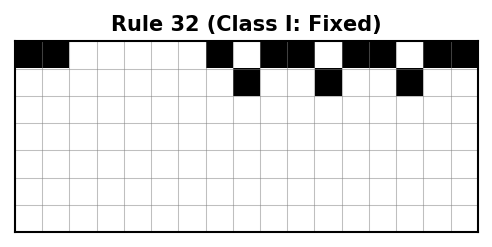
\includegraphics[width=\textwidth]{media/tested_rule_rollouts/rule_032_class_I.png}\\[0.3em]
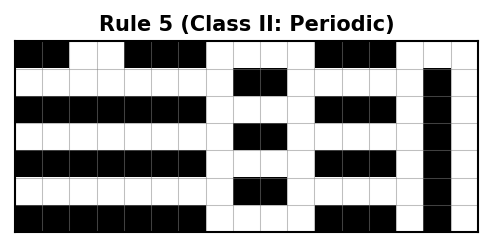
\includegraphics[width=\textwidth]{media/tested_rule_rollouts/rule_005_class_II.png}\\[0.3em]
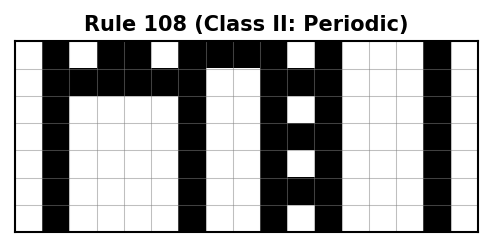
\includegraphics[width=\textwidth]{media/tested_rule_rollouts/rule_108_class_II.png}\\[0.3em]
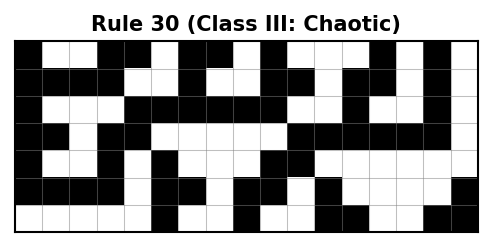
\includegraphics[width=\textwidth]{media/tested_rule_rollouts/rule_030_class_III.png}
\end{minipage}
&
% Column 2: 3 rules
\begin{minipage}{0.48\columnwidth}
\centering
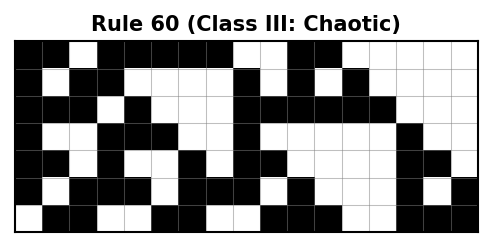
\includegraphics[width=\textwidth]{media/tested_rule_rollouts/rule_060_class_III.png}\\[0.3em]
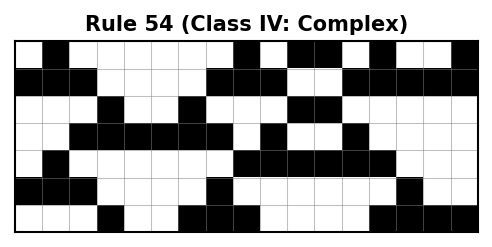
\includegraphics[width=\textwidth]{media/tested_rule_rollouts/rule_054_class_IV.png}\\[0.3em]
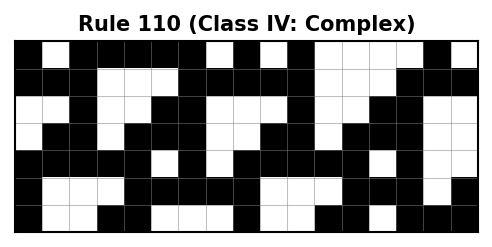
\includegraphics[width=\textwidth]{media/tested_rule_rollouts/rule_110_class_IV.png}
\end{minipage}
\end{tabular}
\end{center}
\caption{Complete spacetime evolutions for all seven CA rules tested in the experiment. Each panel shows the initial row plus 6 time steps of evolution (17 cells wide $\times$ 7 rows). Rules are grouped by Wolfram class: Class I (Rule 32) evolves to a fixed state; Class II (Rules 5, 108) produces periodic structures; Class III (Rules 30, 60) generates chaotic patterns; Class IV (Rules 54, 110) exhibits complex, localized structures.}
\label{fig:all_rollouts}
\end{figure}

\end{document}
